\appendix

\section{Appendix: Experimental Material}
\begin{figure}[ht]
    \centering
    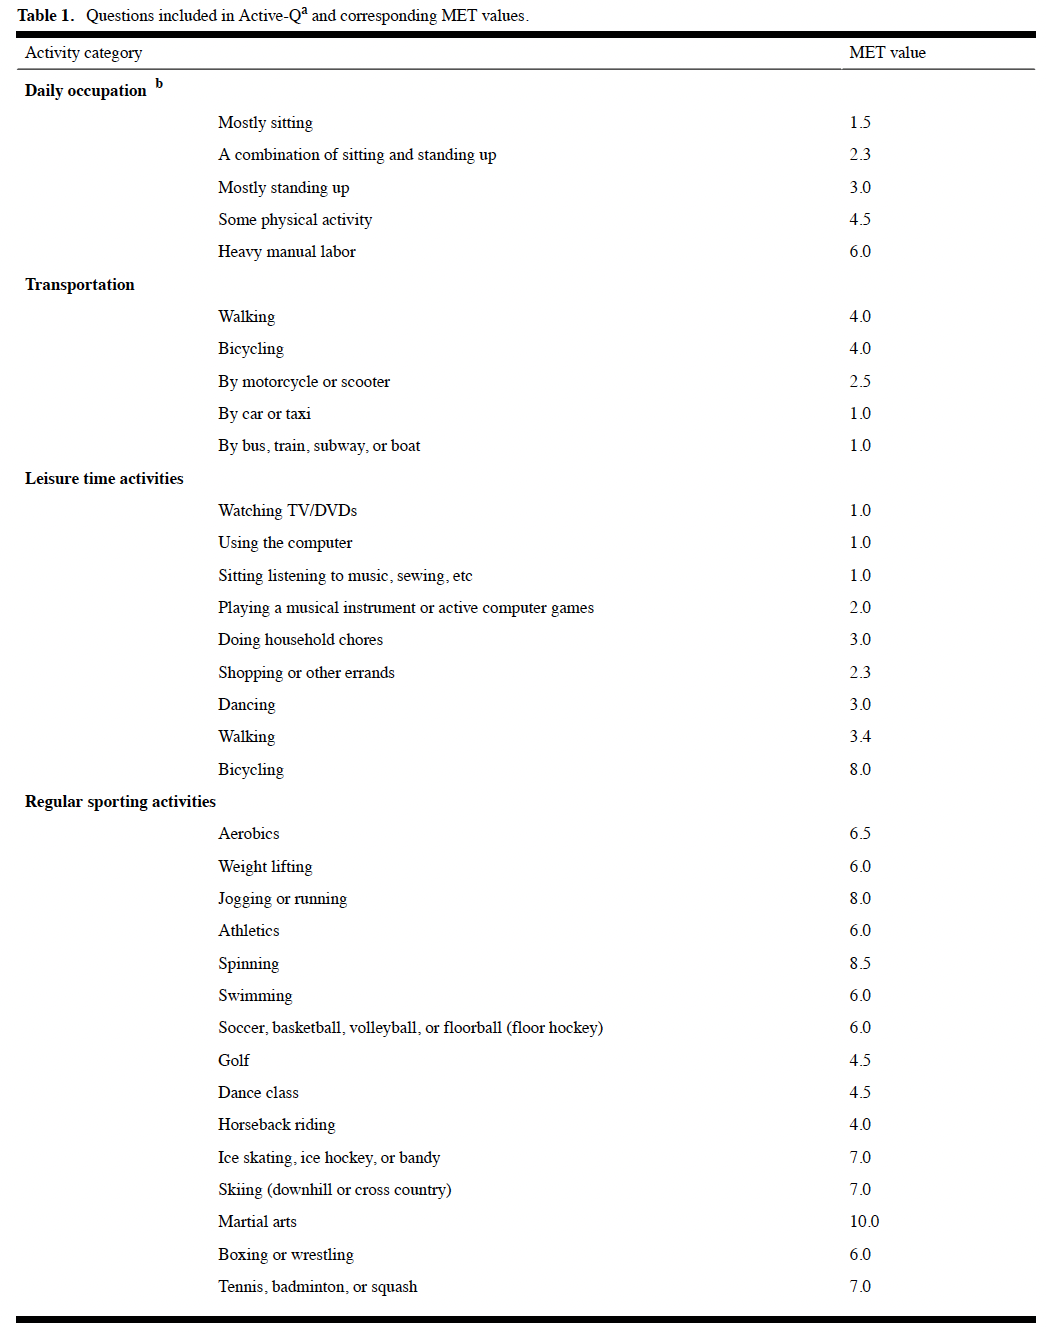
\includegraphics[width=0.8\textwidth]{appendix/met_values.png}
    \caption{MET value labels \parencite{Bonn_2012}}
    \label{fig: met_values}
\end{figure}
\begin{figure}[ht]
    \centering
    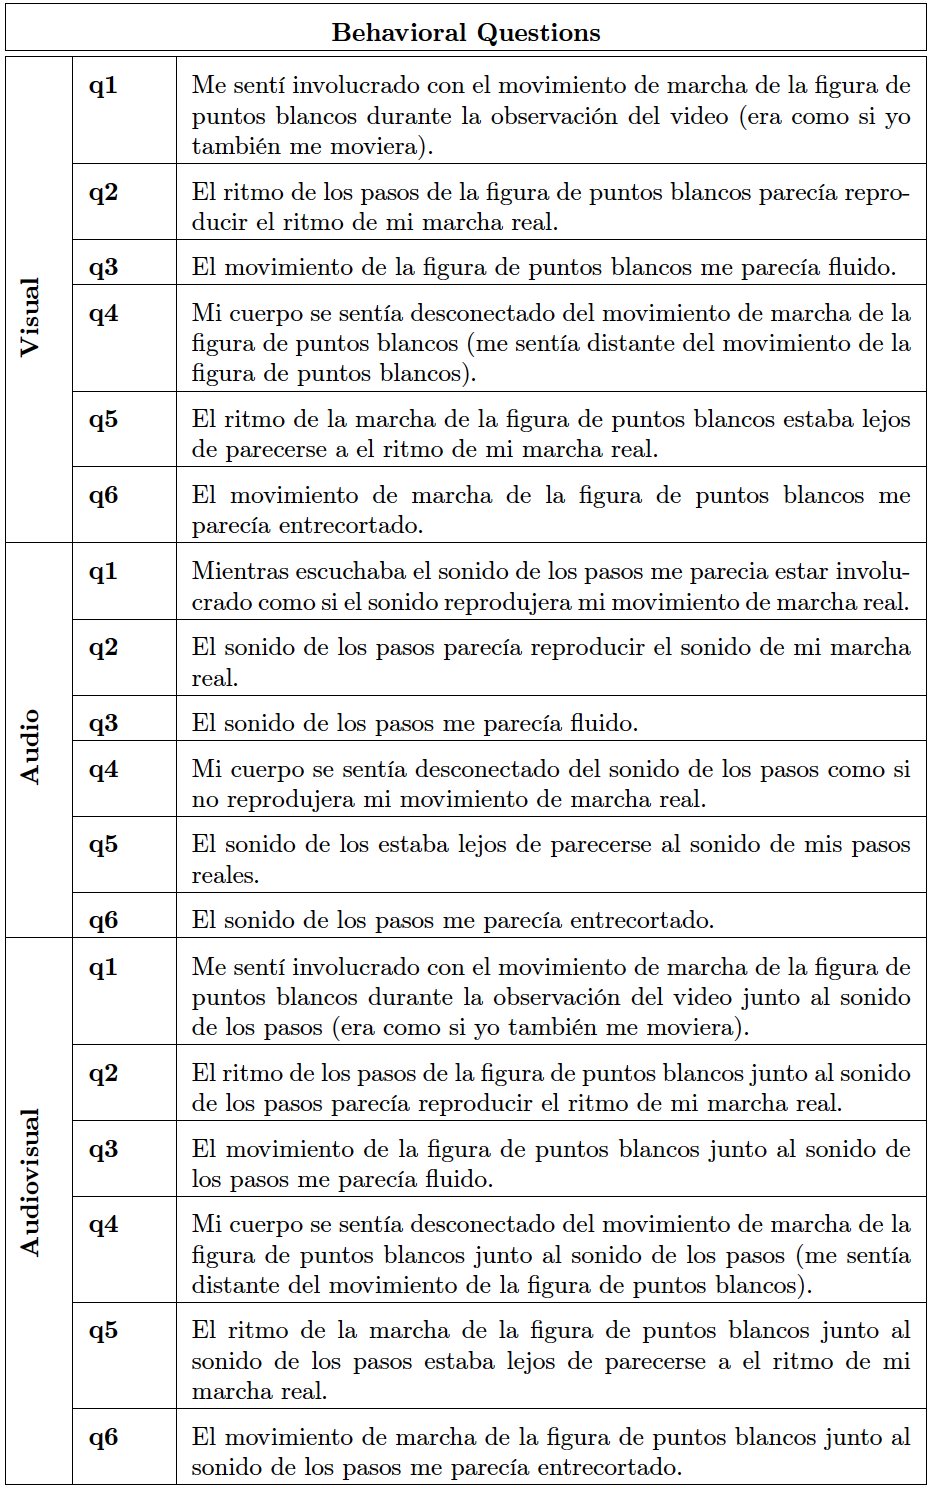
\includegraphics[width=0.70\textwidth]{appendix/questions.png}
    \caption{Behavioral questions translated in English from Spanish}
    \label{fig: Behavioral questions}
\end{figure}
\begin{figure}[ht]
    \centering
    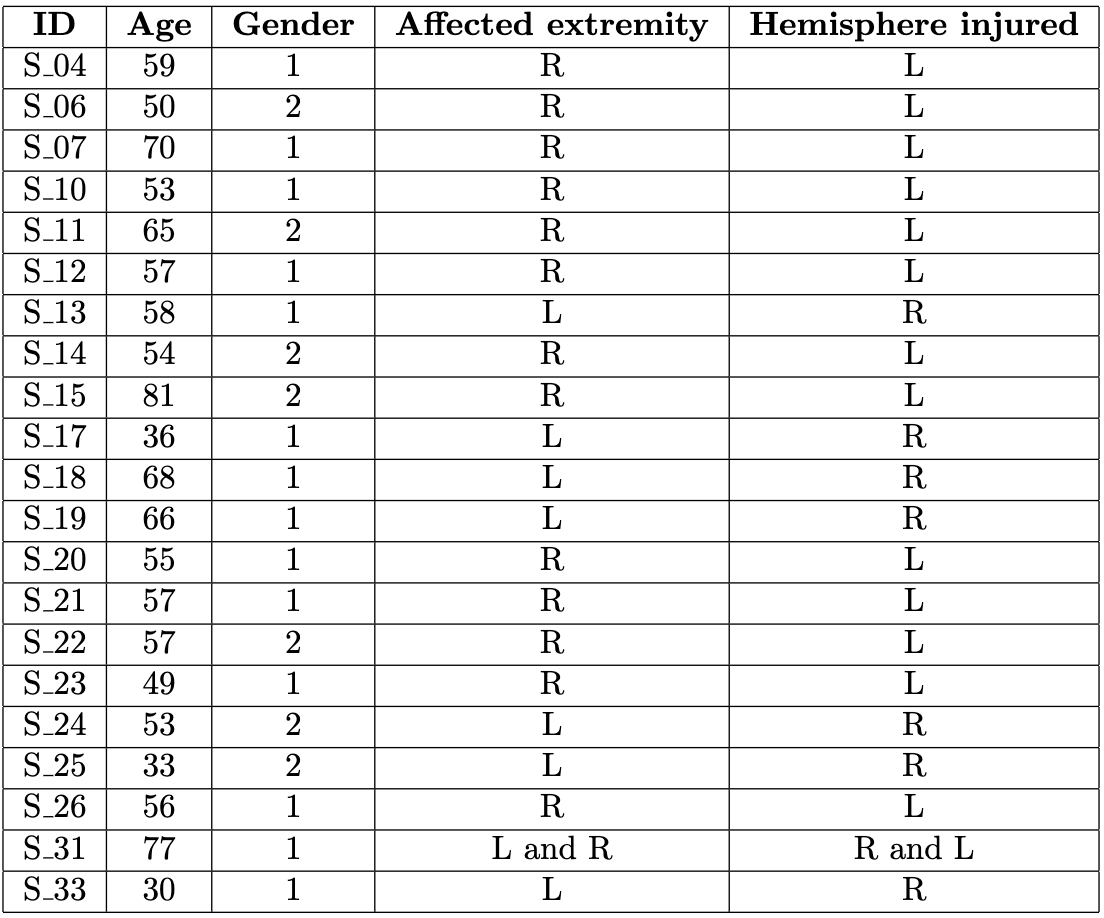
\includegraphics[width=0.70\textwidth]{appendix/database_stroke.png}
    \caption{Database for stroke population (Gender: 1 = man; 2 = woman) }
    \label{fig: Database stroke}
\end{figure}

\clearpage
% \section{Appendix: Active-Q Questionnaire}
% \label{pdf: Active-Q questionnaire}
\includepdf[scale=0.8, pages=1, 
    pagecommand={\section{Appendix: Active-Q questionnaire}\label{pdf: Active-Q questionnaire}}]{appendix/Active-Q test.pdf}
\includepdf[scale=0.8, pages=2-, 
    pagecommand={}]{appendix/Active-Q test.pdf}

\clearpage